\documentclass[11pt]{article}
%Gummi|061|=)
\usepackage{hyperref}
\usepackage[spanish]{babel}
\usepackage[utf8]{inputenc}
\usepackage{pdfpages}
\title{\textbf{RUP: Klondike}}
\author{Israel Pavón Maculet,
Sergio Arroutbi Braojos}
\selectlanguage{spanish}
\date{\today}
%\addtolength{\topmargin}{-0.5in}
\usepackage[bottom=14em]{geometry}
\usepackage{amsmath}
\usepackage{mathtools}
\usepackage{pdflscape}
\usepackage{float}

\begin{document}

\hypersetup
{   
pdfborder={0 0 0}
}
   
\maketitle

\pagebreak

\tableofcontents

\pagebreak

\section{Introducción}
En este ejercicio se han implementado diversos diagramas de los modelos del dominio, caso de uso y análisis del juego del klondike. Este juego de cartas, también conocido como ``solitario'', es un juego en el que un único jugador interviene en el reparto y el posterior manejo y posicionamiento de las cartas.

Para realizar la implementación software de este juego de cartas se han realizado las diversas fases involucradas en el proceso de desarrollo unificado con diseño orientado a objetos, para el cual se han seguido las siguientes fases:

\begin{itemize}\itemsep0pt
\item{Modelo del Dominio}
\item{Modelo de Casos de Uso}
\item{Modelo de Análisis}
\end{itemize}

En los siguientes capítulos se describen cada una de los anteriores modelos y la aproximación que se ha llevado a cabo con el objetivo de llegar a la fase de diseño y posterior implementacion con todos los artefactos necesarios que aseguren que se lleven a cabo de la mejor forma possible.

\pagebreak

\section{Modelo del Dominio}

El modelo del dominio es una aproximación al problema que se desea implementar desde un punto de vista del dominio real de la aplicación, esto es, obviando que existe software.

En este caso, el modelo del dominio se caracteriza por las características del juego klondike a nivel de juego de cartas exclusivamente, esto es, cómo jugaría un humano si tuviera cartas físicas en su mano y jugara una partida en esta modalidad. 

Dicho lo anterior, hay que clarificar que la disposición de las cartas está formada por la baraja inicial, conocida como ``Deck'', el ``Waste'', donde se levantan las cartas de la baraja, una serie de ``Tableaus'', que permiten sacar de forma provisional las cartas del ``Waste'' ordenándolas por número descendente y alternando los colores de las cartas, y finalmente las ``Foundations'', que son cada uno de los palos del ``Deck'' en orden ascendente.

En cada turno, el jugador puede sacar cartas del ``Deck'' al ``Waste'', colocar cartas del ``Waste'' a los ``Tableaus'' o a las ``Foundations'' y sacar igualmente carta de las ``Foundations'' para seguir combinando cartas en los ``Tableaus''.

Este documento no busca describir de forma muy detallada el juego, que puede consultarse en el siguiente enlace: \url{https://en.wikipedia.org/wiki/Klondike_(solitaire)}

Sin embargo, en el modelo del dominio sí que se recomienda elaborar algunos diagramas que permitan especificar los detalles más importantes del juego.

Así, para el juego del Klondike, se pueden especificar algunos diagramas que permiten mostrar las características básicas del juego.

Para comenzar, hay que explicar el funcionamiento del juego desde el punto de vista de las acciones básicas que lleva a cabo el jugador, expresadas a través del siguiente diagrama:

\begin{center}
 \begin{figure}[H]
 \begin{center}
   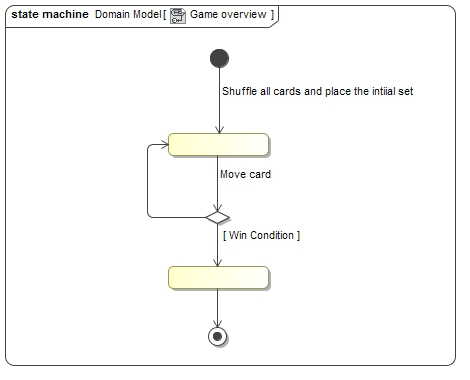
\includegraphics[width=15cm]{DomainModel/GameOverview00.jpg}
   \caption{Funcionamiento básico}
   \label{fig:gamebasics}
 \end{center}
 \end{figure}
\end{center}

En segundo lugar, se identifican los tipos de mazos involucrados en el juego, esto es, las cartas y los tipos de mazos de cartas que se compondrán:

\begin{center}
 \begin{figure}[H]
 \begin{center}
   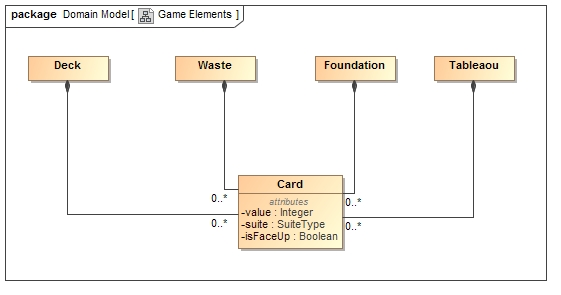
\includegraphics[width=15cm]{DomainModel/GameElements00.jpg}
   \caption{Elementos del Juego}
   \label{fig:gamelements}
 \end{center}
 \end{figure}
\end{center}

Además de los tipos de objetos tangibles existentes en el juego, es reseñable el ciclo de vida por el que pasa una carta en el transcurso del juego, como muestra el siguiente diagrama:

\begin{center}
 \begin{figure}[H]
 \begin{center}
   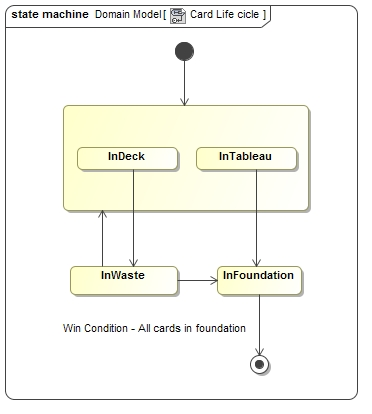
\includegraphics[width=10cm]{DomainModel/CardLifeCycle00.jpg}
   \caption{Ciclo de vida de una carta}
   \label{fig:cardlifecycle}
 \end{center}
 \end{figure}
\end{center}

Y en cuanto a la disposición de los elementos en el juego, es decir, qué mazos contienen qué cartas y en qué estado en el reparto inicial de las mismas, se propone el siguiente diagrama:

\begin{center}
 \begin{figure}[H]
 \begin{center}
   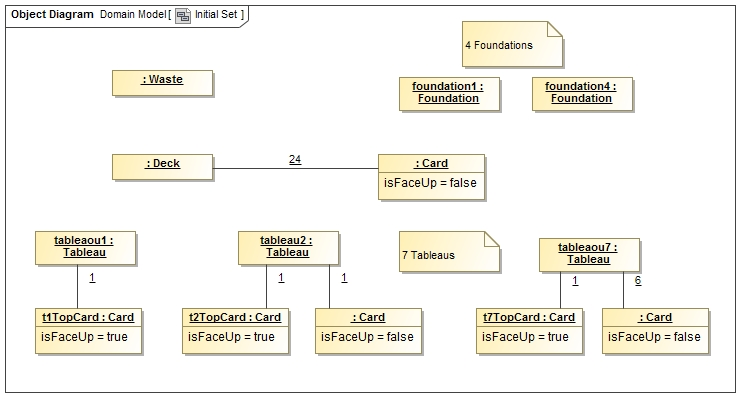
\includegraphics[width=16cm]{DomainModel/InitialSet00.jpg}
   \caption{Disposición Inicial}
   \label{fig:initialset}
 \end{center}
 \end{figure}
\end{center}

Una vez descritos los objetos presentes en el juego, su relación de composición su posicionamiento inicial, cabe destacar que a nivel de modelo del dominio hay que documentar cada uno de los tipos de movimientos posibles en el juego por separado, ya que hacerlo todo a través de un mismo diagrama podría resultar bastante complejo de comprender. Así, se proponen los siguientes diagramas para cada uno de los movimientos:

\begin{center}
 \begin{figure}[H]
 \begin{center}
   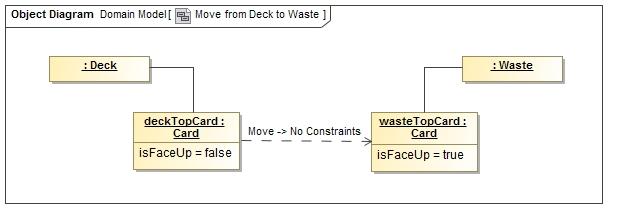
\includegraphics[width=15cm]{DomainModel/MoveFromDeckToWaste00.jpg}
   \caption{Move From Deck To Waste}
   \label{fig:deck2waste}
 \end{center}
 \end{figure}
\end{center}

\begin{center}
 \begin{figure}[H]
 \begin{center}
   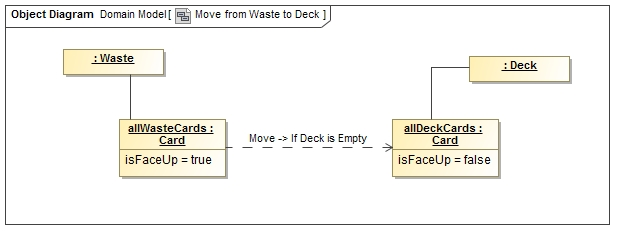
\includegraphics[width=15cm]{DomainModel/MoveFromWasteToDeck00.jpg}
   \caption{Move From Waste To Deck}
   \label{fig:waste2deck}
 \end{center}
 \end{figure}
\end{center}

\begin{center}
 \begin{figure}[H]
 \begin{center}
   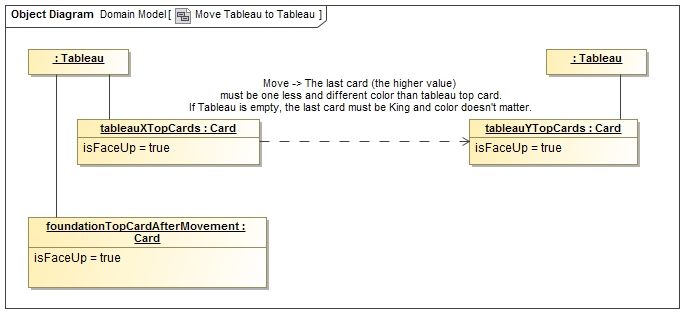
\includegraphics[width=15cm]{DomainModel/MoveTableauToTableau00.jpg}
   \caption{Move From Tableau To Tableau}
   \label{fig:tableautotableau}
 \end{center}
 \end{figure}
\end{center}

\begin{center}
 \begin{figure}[H]
 \begin{center}
   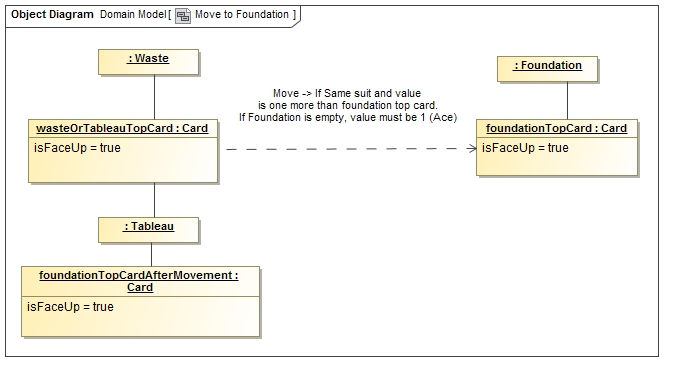
\includegraphics[width=15cm]{DomainModel/MoveToFoundation00.jpg}
   \caption{Move To Foundation}
   \label{fig:tofoundation}
 \end{center}
 \end{figure}
\end{center}

\begin{center}
 \begin{figure}[H]
 \begin{center}
   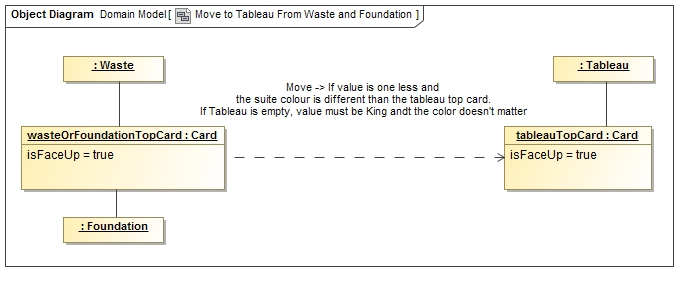
\includegraphics[width=15cm]{DomainModel/MoveToTableauFromWasteAndFoundation00.jpg}
   \caption{Move To Tableau From Waste Or Foundation}
   \label{fig:totableaufromwasteorfoundation}
 \end{center}
 \end{figure}
\end{center}

Los anteriores diagramas de estados y de objetos permiten establecer una primera aproximación al juego del Klondike, a través de las nociones más básicas del juego.

En los apartados posteriores se establecerán los casos de uso identificados en el modelo de casos de uso, así como el modelo de análisis con las clases resultantes de esta fase.

\pagebreak

\section{Modelo de Casos de Uso}

Una vez conocida la funcionalidad básica del juego, se identifican cuatro casos de uso básicos en la aplicación, definidos por el siguiente diagrama:

\begin{center}
 \begin{figure}[H]
 \begin{center}
   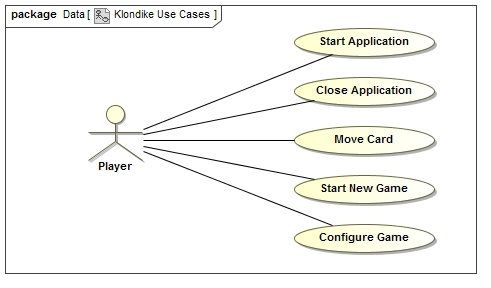
\includegraphics[width=15cm]{DomainModel/KlondikeUseCases02.jpg}
   \caption{Casos de uso}
   \label{fig:usecases}
 \end{center}
 \end{figure}
\end{center}

A su vez, el diagrama que muestra la relación entre los distintos casos de uso puede observarse en el siguiente diagrama:

\begin{center}
 \begin{figure}[H]
 \begin{center}
   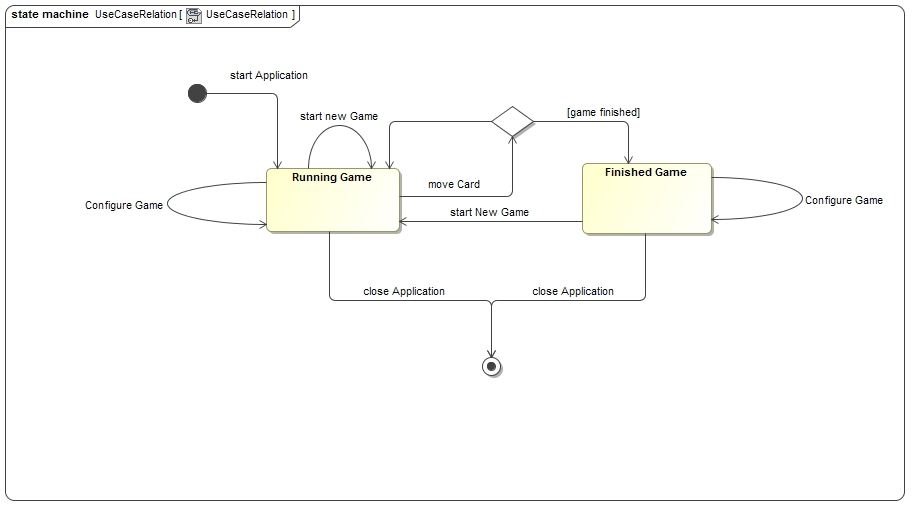
\includegraphics[width=16cm]{DomainModel/UseCaseRelation01.jpg}
   \caption{Relación entre casos de uso}
   \label{fig:usecaserelation}
 \end{center}
 \end{figure}
\end{center}

Una vez encontrados los casos de uso y propuesta la relación existente entre ellos, cabe mencionar que el paso siguiente es priorizar los casos de uso.

En este caso, los casos de uso con más riesgo (contemplando todo tipo de riesgos como puedan ser riesgos tecnológicos, de computación, etc.) se considera que son los casos de ``Start New Game'' y ``Move Card'':

\begin{center}
 \begin{figure}[H]
 \begin{center}
   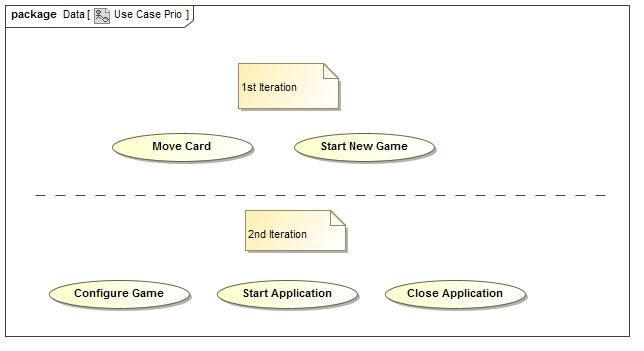
\includegraphics[width=15cm]{DomainModel/UseCasePrio02.jpg}
   \caption{Priorización de los casos de uso}
   \label{fig:usecasepriorization}
 \end{center}
 \end{figure}
\end{center}


El caso de uso ``Start Game'' se describe a través del siguiente diagrama de estados:

\begin{center}
 \begin{figure}[H]
 \begin{center}
   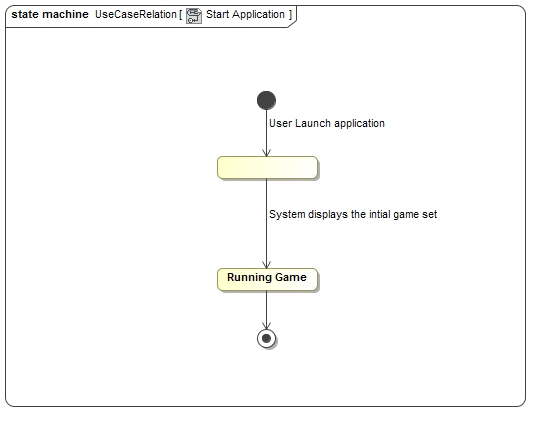
\includegraphics[width=15cm]{DomainModel/StartApplication00.jpg}
   \caption{Arrancar Aplicación}
   \label{fig:startapplication}
 \end{center}
 \end{figure}
\end{center}

Por otro lado, el caso de uso ``Start New Game'' hace referencia al reparto de las cartas, tanto si es el reparto inicial como si es un reparto que el jugador realiza en mitad de la partida, puesto que quiere comenzar la partida de nuevo. Puede observarse este caso de uso a través del siguiente diagrama:

\begin{center}
 \begin{figure}[H]
 \begin{center}
   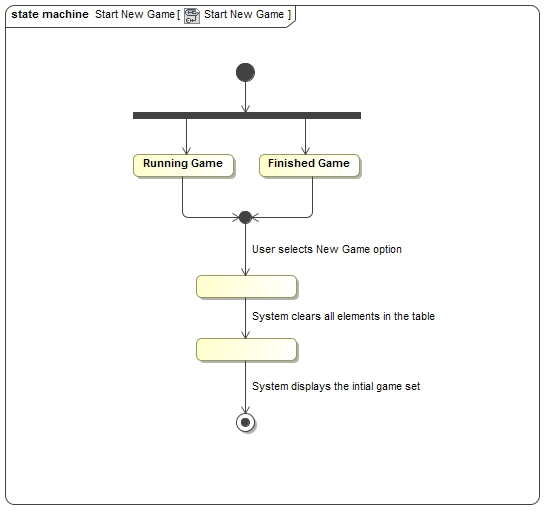
\includegraphics[width=15cm]{DomainModel/StartNewGame00.jpg}
   \caption{Comenzar Juego}
   \label{fig:startnewgame}
 \end{center}
 \end{figure}
\end{center}

Otro caso de uso identificado es aquél que permite a un usuario realizar cambios en la configuración del juego, en parámetros como el tipo de baraja a utilizar, el modo en que se pasan las cartas del Waste al Deck, etc.etc.etc. Dicho caso de uso queda reflejado a través del siguiente diagrama de estados:

\begin{center}
 \begin{figure}[H]
 \begin{center}
   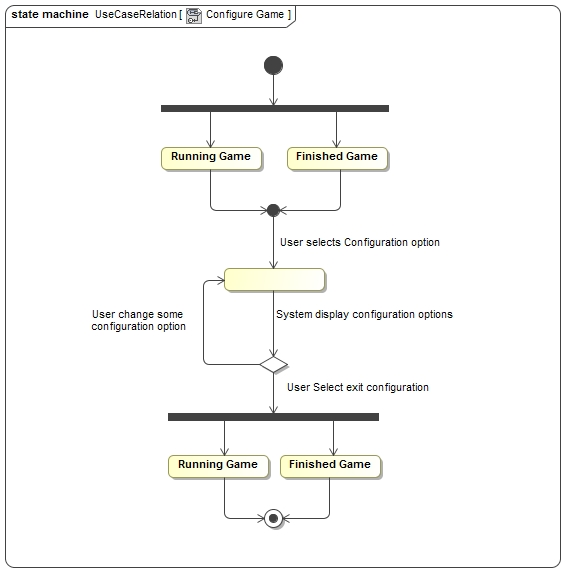
\includegraphics[width=17cm]{DomainModel/ConfigureGame00.jpg}
   \caption{Comenzar Juego}
   \label{fig:startnewgame}
 \end{center}
 \end{figure}
\end{center}

Finalmente, el caso de uso ``Close Application'' hace referencia al cierre de la aplicación por parte del usuario, como muestra el siguiente diagrama:

\begin{center}
 \begin{figure}[H]
 \begin{center}
   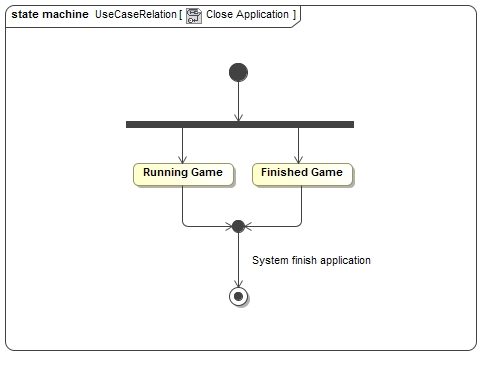
\includegraphics[width=15cm]{DomainModel/CloseApplication00.jpg}
   \caption{Finalizar Juego}
   \label{fig:finishgame}
 \end{center}
 \end{figure}
\end{center}

Los casos de uso de arranque de la aplicación, reparto de cartas o fin de partida no merecen desarrollo adicional en cuanto a los diagramas que los representan, ya que son casos muy claros una vez conocido el funcionamiento del juego. Sin embargo, el modelo de casos de uso debe hacer hincapié en qué pasa cuando se posiciona una carta desde un mazo a otro dentro del juego.

En primer lugar, cabe indicar que hay una jerarquía de movimientos disponible dentro de este juego de cartas. De esta forma, se identifica el siguiente diagrama, que permite establecer, dentro del caso de uso ``Move Card'', los distintos tipos de movimientos posibles. Pueden observarse en la siguiente figura:

\begin{center}
 \begin{figure}[H]
 \begin{center}
   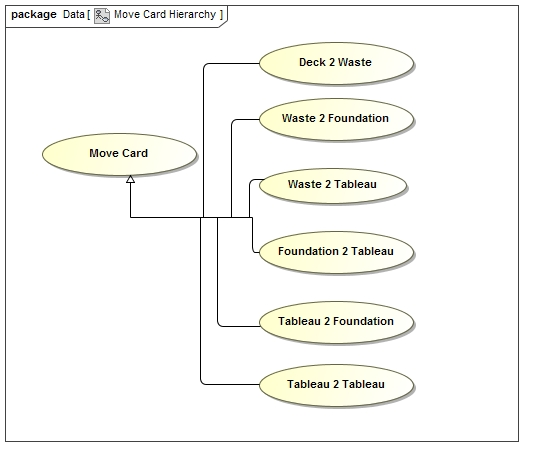
\includegraphics[width=15cm]{DomainModel/MoveCardHierarchy.jpg}
   \caption{Movimientos}
   \label{fig:movements}
 \end{center}
 \end{figure}
\end{center}

Una vez identificados los posibles movimientos, la realización de cada uno de los movimientos puede definirse como subacciones de ``Move Card''.

Una forma de especificar qué ocurre dentro de cada uno de los distintos movimientos es a través de diagramas de estados. A continuación, se muestran los estados que definen el problema del dominio para cada uno de los movimientos:

\begin{center}
 \begin{figure}[H]
 \begin{center}
   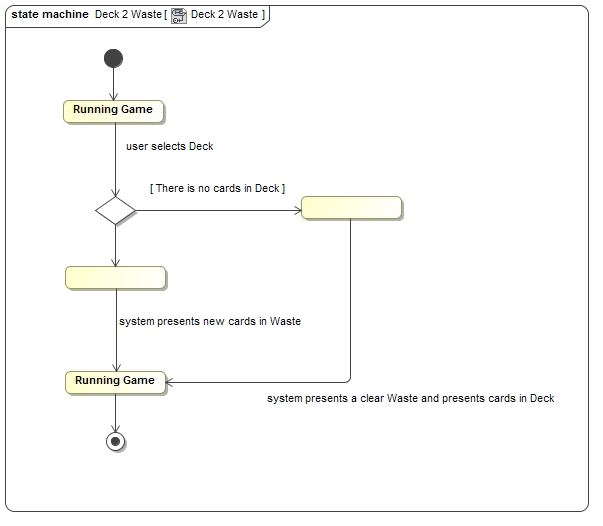
\includegraphics[width=15cm]{DomainModel/Deck2Waste.jpg}
   \caption{Deck To Waste}
   \label{fig:deck2waste}
 \end{center}
 \end{figure}
\end{center}
\begin{center}

\begin{figure}[H]
 \begin{center}
   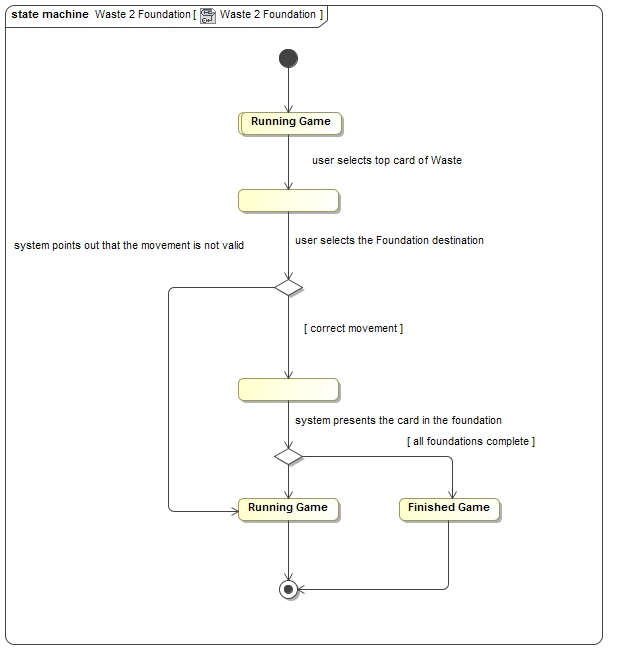
\includegraphics[width=15cm]{DomainModel/Waste2Foundation.jpg}
   \caption{Waste To Foundation}
   \label{fig:waste2foundation}
 \end{center}
 \end{figure}
\end{center}

\begin{center}
 \begin{figure}[H]
 \begin{center}
   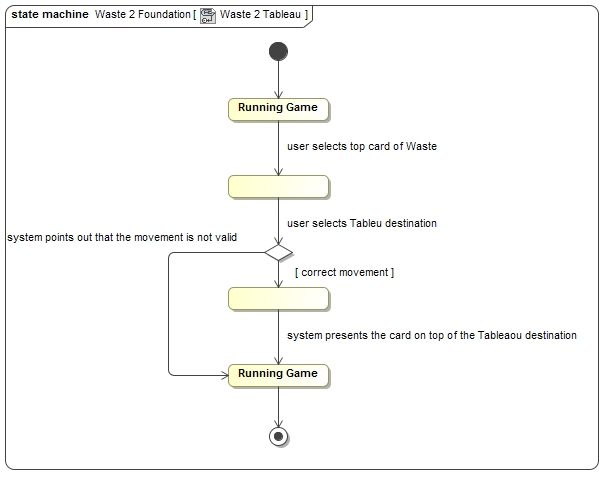
\includegraphics[width=15cm]{DomainModel/Waste2Tableau.jpg}
   \caption{Waste To Tableau}
   \label{fig:waste2tableau}
 \end{center}
 \end{figure}
\end{center}

\begin{center}
 \begin{figure}[H]
 \begin{center}
   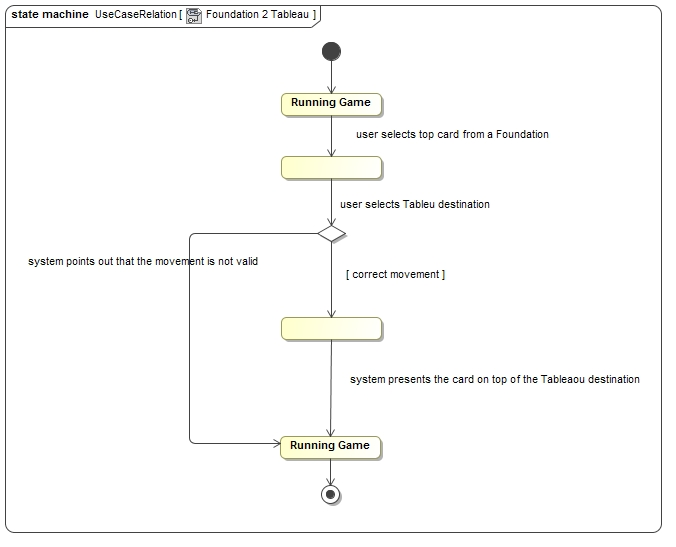
\includegraphics[width=15cm]{DomainModel/Foundation2Tableau.jpg}
   \caption{Foundation To Tableau}
   \label{fig:foundation2tableau}
 \end{center}
 \end{figure}
\end{center}

\begin{center}
 \begin{figure}[H]
 \begin{center}
   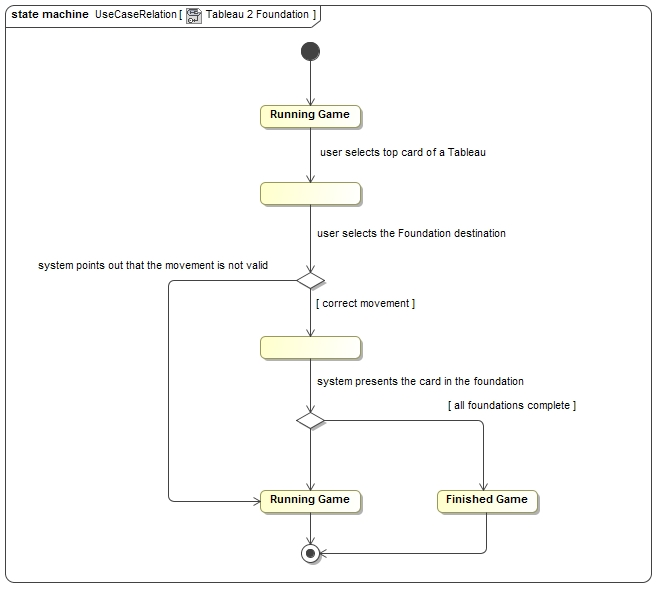
\includegraphics[width=15cm]{DomainModel/Tableau2Foundation.jpg}
   \caption{Tableau To Foundation}
   \label{fig:tableau2foundation}
 \end{center}
 \end{figure}
\end{center}

\begin{center}
 \begin{figure}[H]
 \begin{center}
   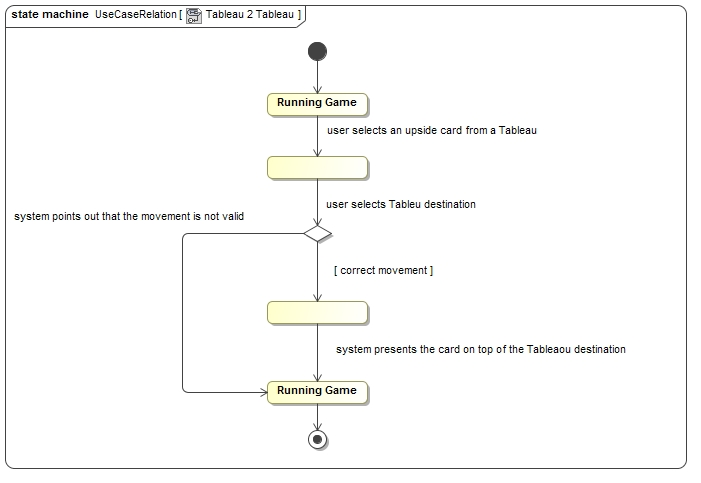
\includegraphics[width=15cm]{DomainModel/Tableau2Tableau.jpg}
   \caption{Tableau To Tableau}
   \label{fig:tableau2tableau}
 \end{center}
 \end{figure}
\end{center}

A través de los diagramas anteriores se ha pretendido realizar una documentación clara y explícita de las condiciones por la que transiciona el sistema por cada uno de los casos de uso, básicamente, a través de diagramas de estado. De esta forma, la fase de análisis se podrá acometer de una manera más natural, ya que empiezan a aparecer conceptos que pueden ser directamente mapeados a clases, como, por ejemplo, los movimientos de las cartas, cada uno de los tipos de mazos que hay involucrados en el juego, etc.

\pagebreak

\section{Modelo de Análisis}

La fase de análisis es, simplemente, un \textbf{``diseño preliminar''}. Se considera que esta fase de análisis se debe de llevar a cabo en una quinta parte del tiempo total respecto a la fase de diseño.

En esta fase de análisis, en la cual la solución al proceso de desarrollo empieza a tomar forma, se debe dar una primera visión interna del sistema, de forma que empiezan a aflorar los primeros diagramas estructurados por clases estereotipadas. Estos diagramas suelen recoger aquellos detalles del dominio propios de los objetos identficados en dicha fase.

Por tanto, en esta fase de análisis se debe empezar a documentar en qué partes se va a descomponer el sistema de forma que se desarrolle una división del problema planteado en diversas clases que tendrán distintas responsabilidades e interactuarán entre sí para llegar a la solución final. 

Por tanto, teniendo en cuenta lo anterior, desde el punto de vista del modelo de análisis, existen dos tipos de diagramas principales que permiten realizar el modelado de la fase de análisis.

\begin{itemize}
\item{Diagramas de Clases}. 
\item{Diagramas de Colaboración entre Clases}.
\end{itemize}

En general, para el modelo de análisis, se deben tomar las clases esbozadas del modelo del dominio junto a la realización de casos de uso del modelo de casos de uso, para obtener un conjunto completo de clases de análisis y la relación de colaboración que existe entre ellas.

Para una mejor clasificación de las clases, es recomendable que éstas se agrupen por casos de uso.

\subsection{Diagramas de Clases}

Así, para el juego del klondike, se han identificado las siguientes clases por caso de uso:

\newgeometry{top=0cm,left=1cm,bottom=0cm}
\begin{landscape}
\begin{center}
 \begin{figure}[H]
 \begin{center}
 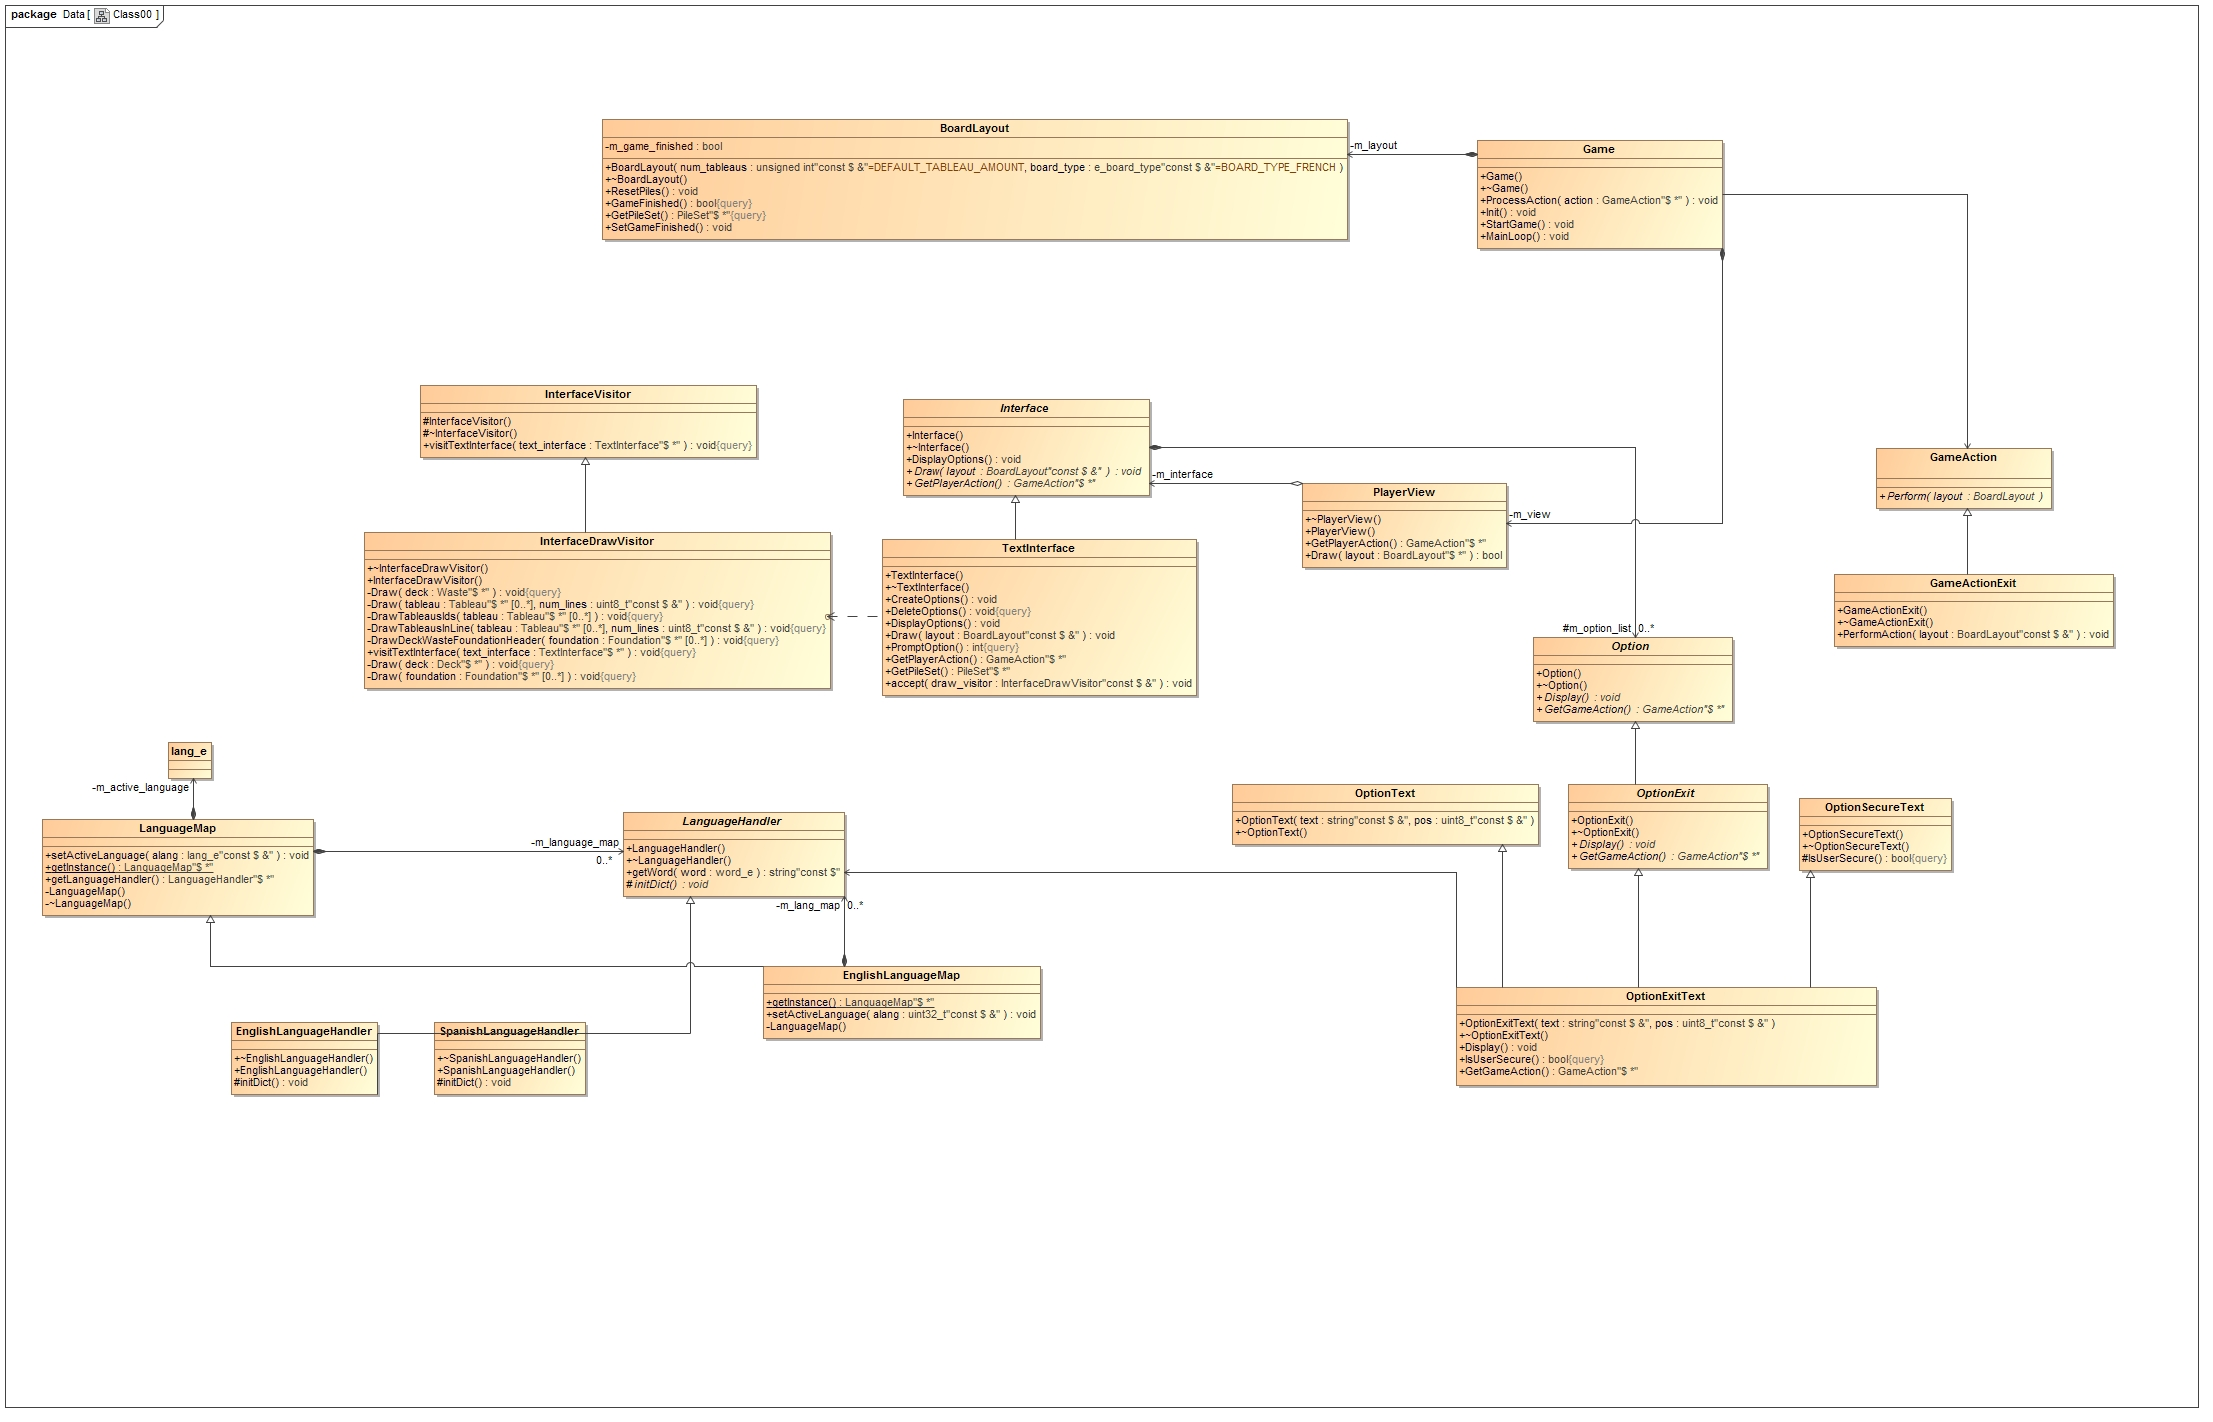
\includegraphics[scale=0.32]{Analysis/ExitGame00.jpg}
   \caption{Diagrama de Clases: ``Exit Game''}
   \label{fig:exitgame}
 \end{center}
 \end{figure}
\end{center}
\end{landscape}
\restoregeometry

\newgeometry{top=0cm,left=1cm,bottom=0cm}
\begin{landscape}
\begin{center}
 \begin{figure}[H]
 \begin{center}
 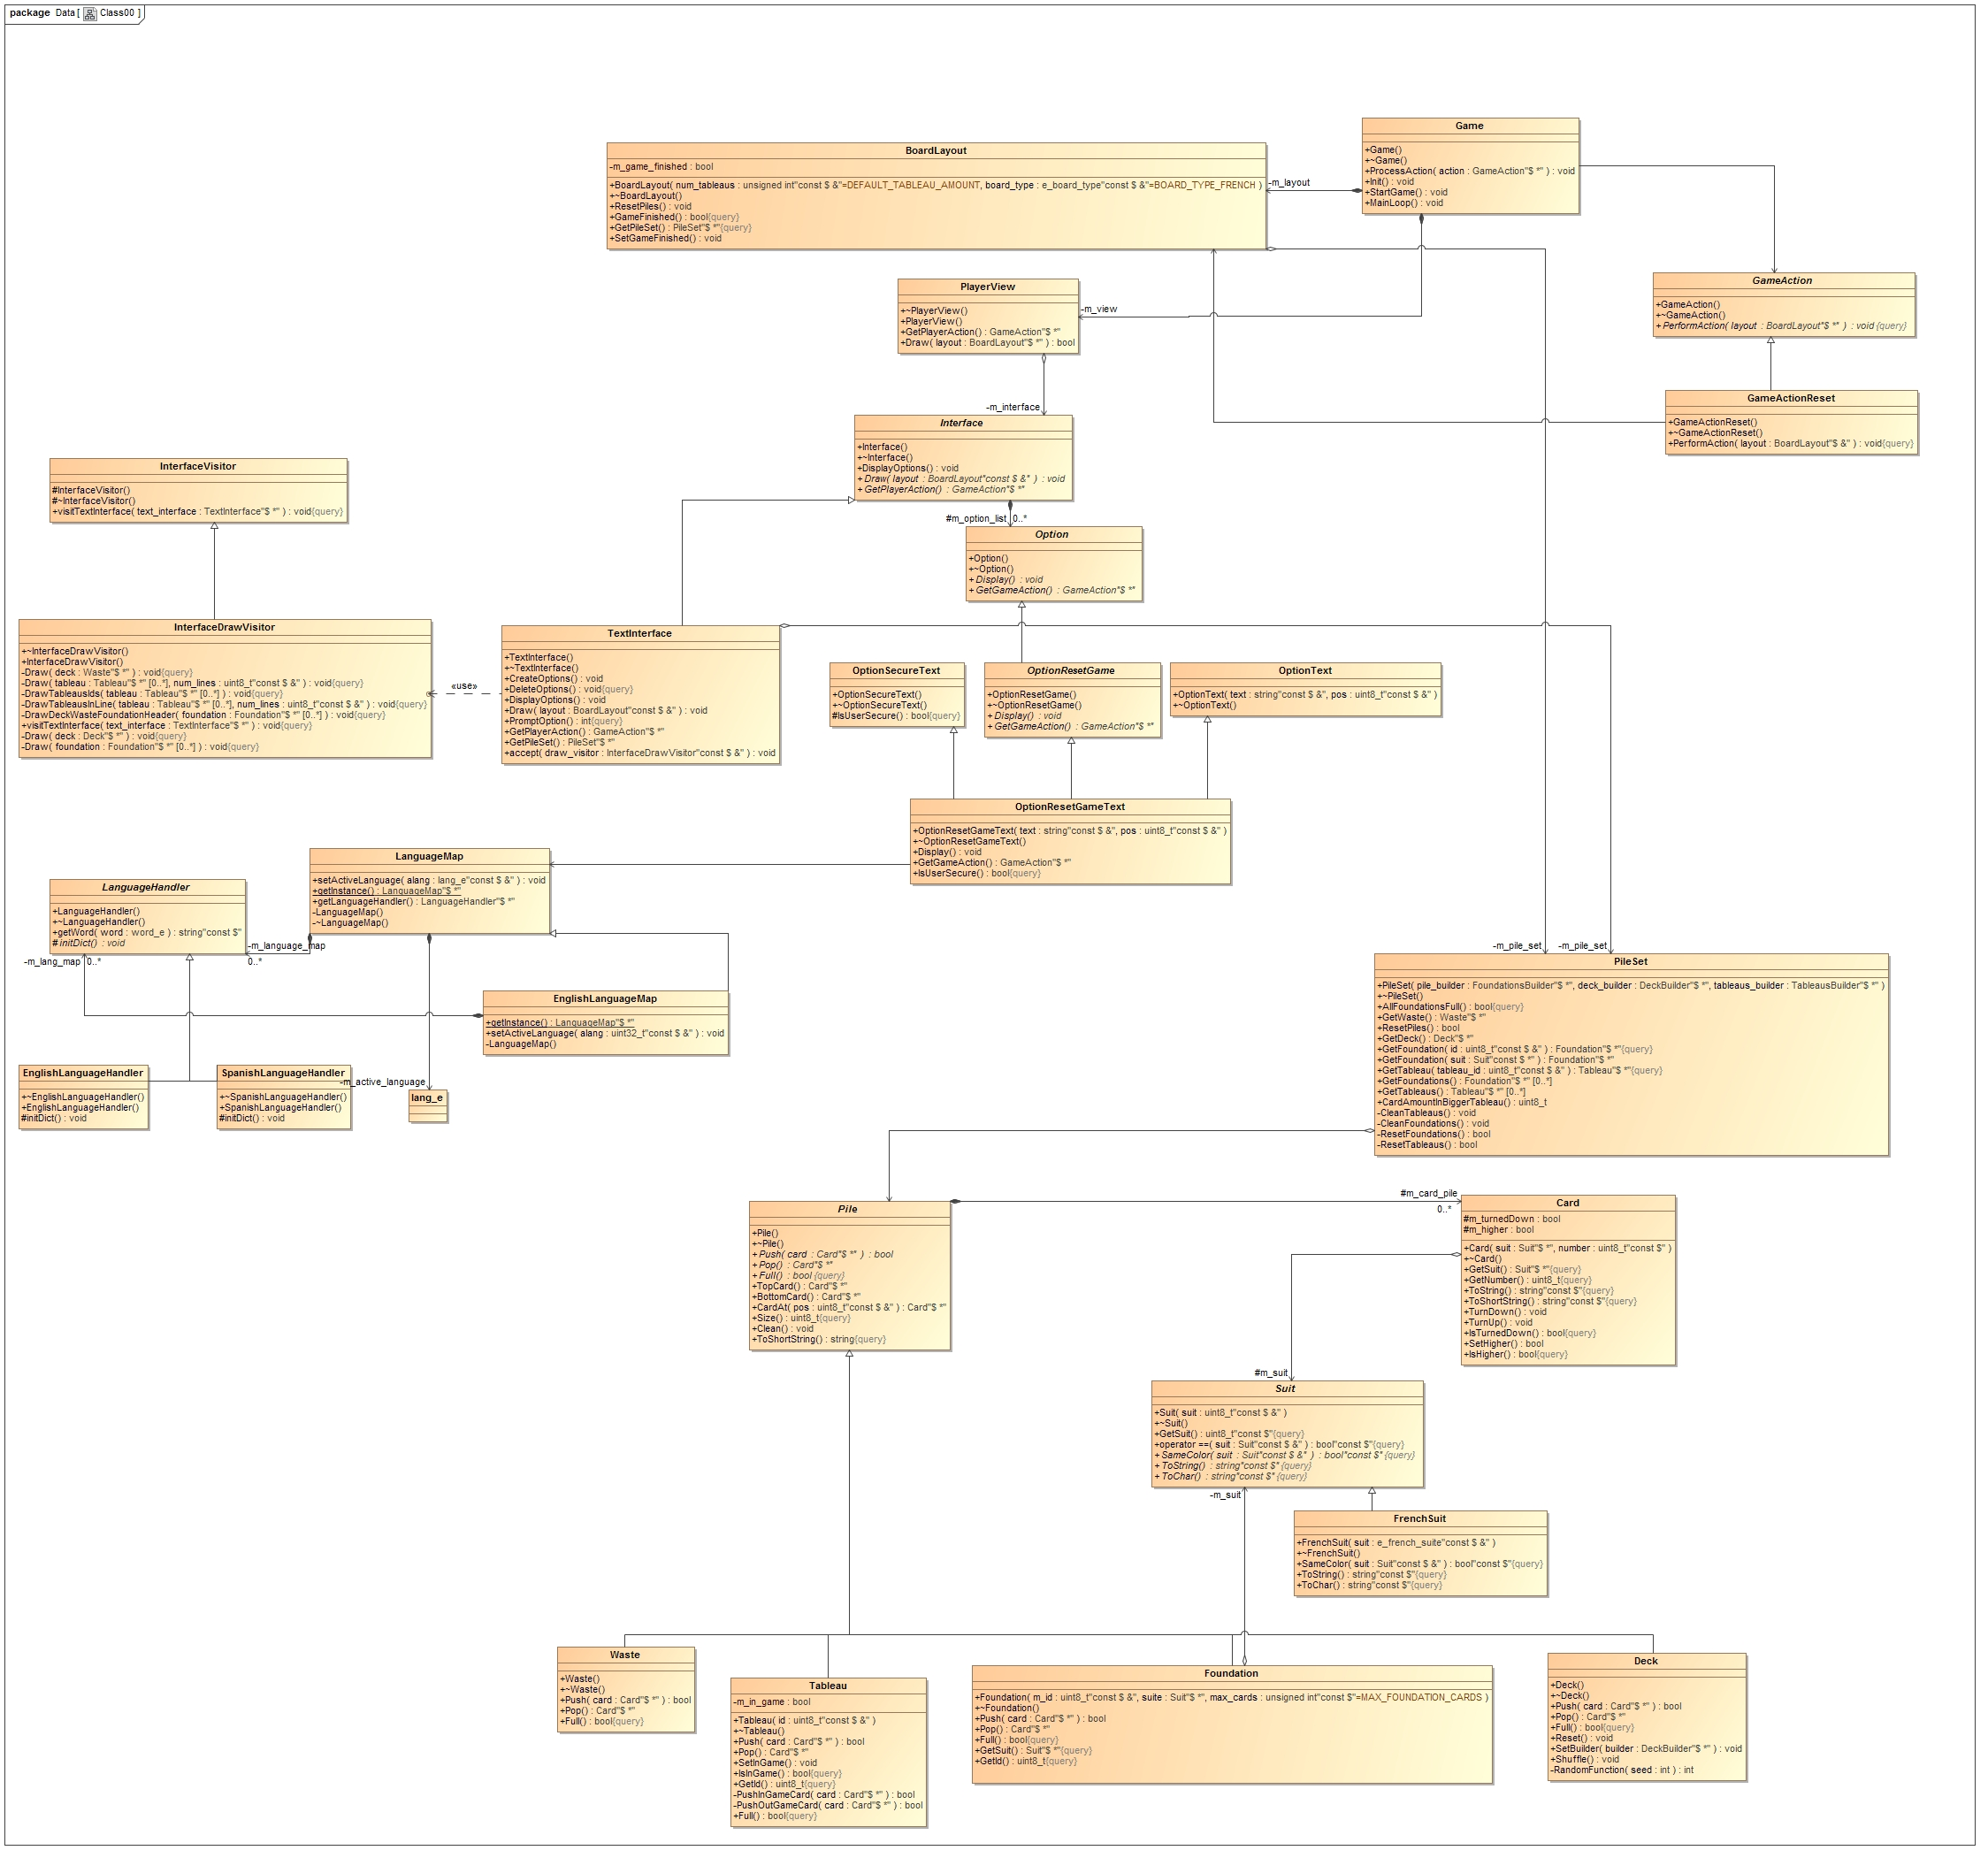
\includegraphics[scale=0.22]{Analysis/ResetGame00.jpg}
   \caption{Diagrama de Clases: ``Start New Game''}
   \label{fig:resetgame}
 \end{center}
 \end{figure}
\end{center}
\end{landscape}
\restoregeometry

\newgeometry{top=0cm,left=1cm,bottom=0cm}
\begin{landscape}
\begin{center}
 \begin{figure}[H]
 \begin{center}
 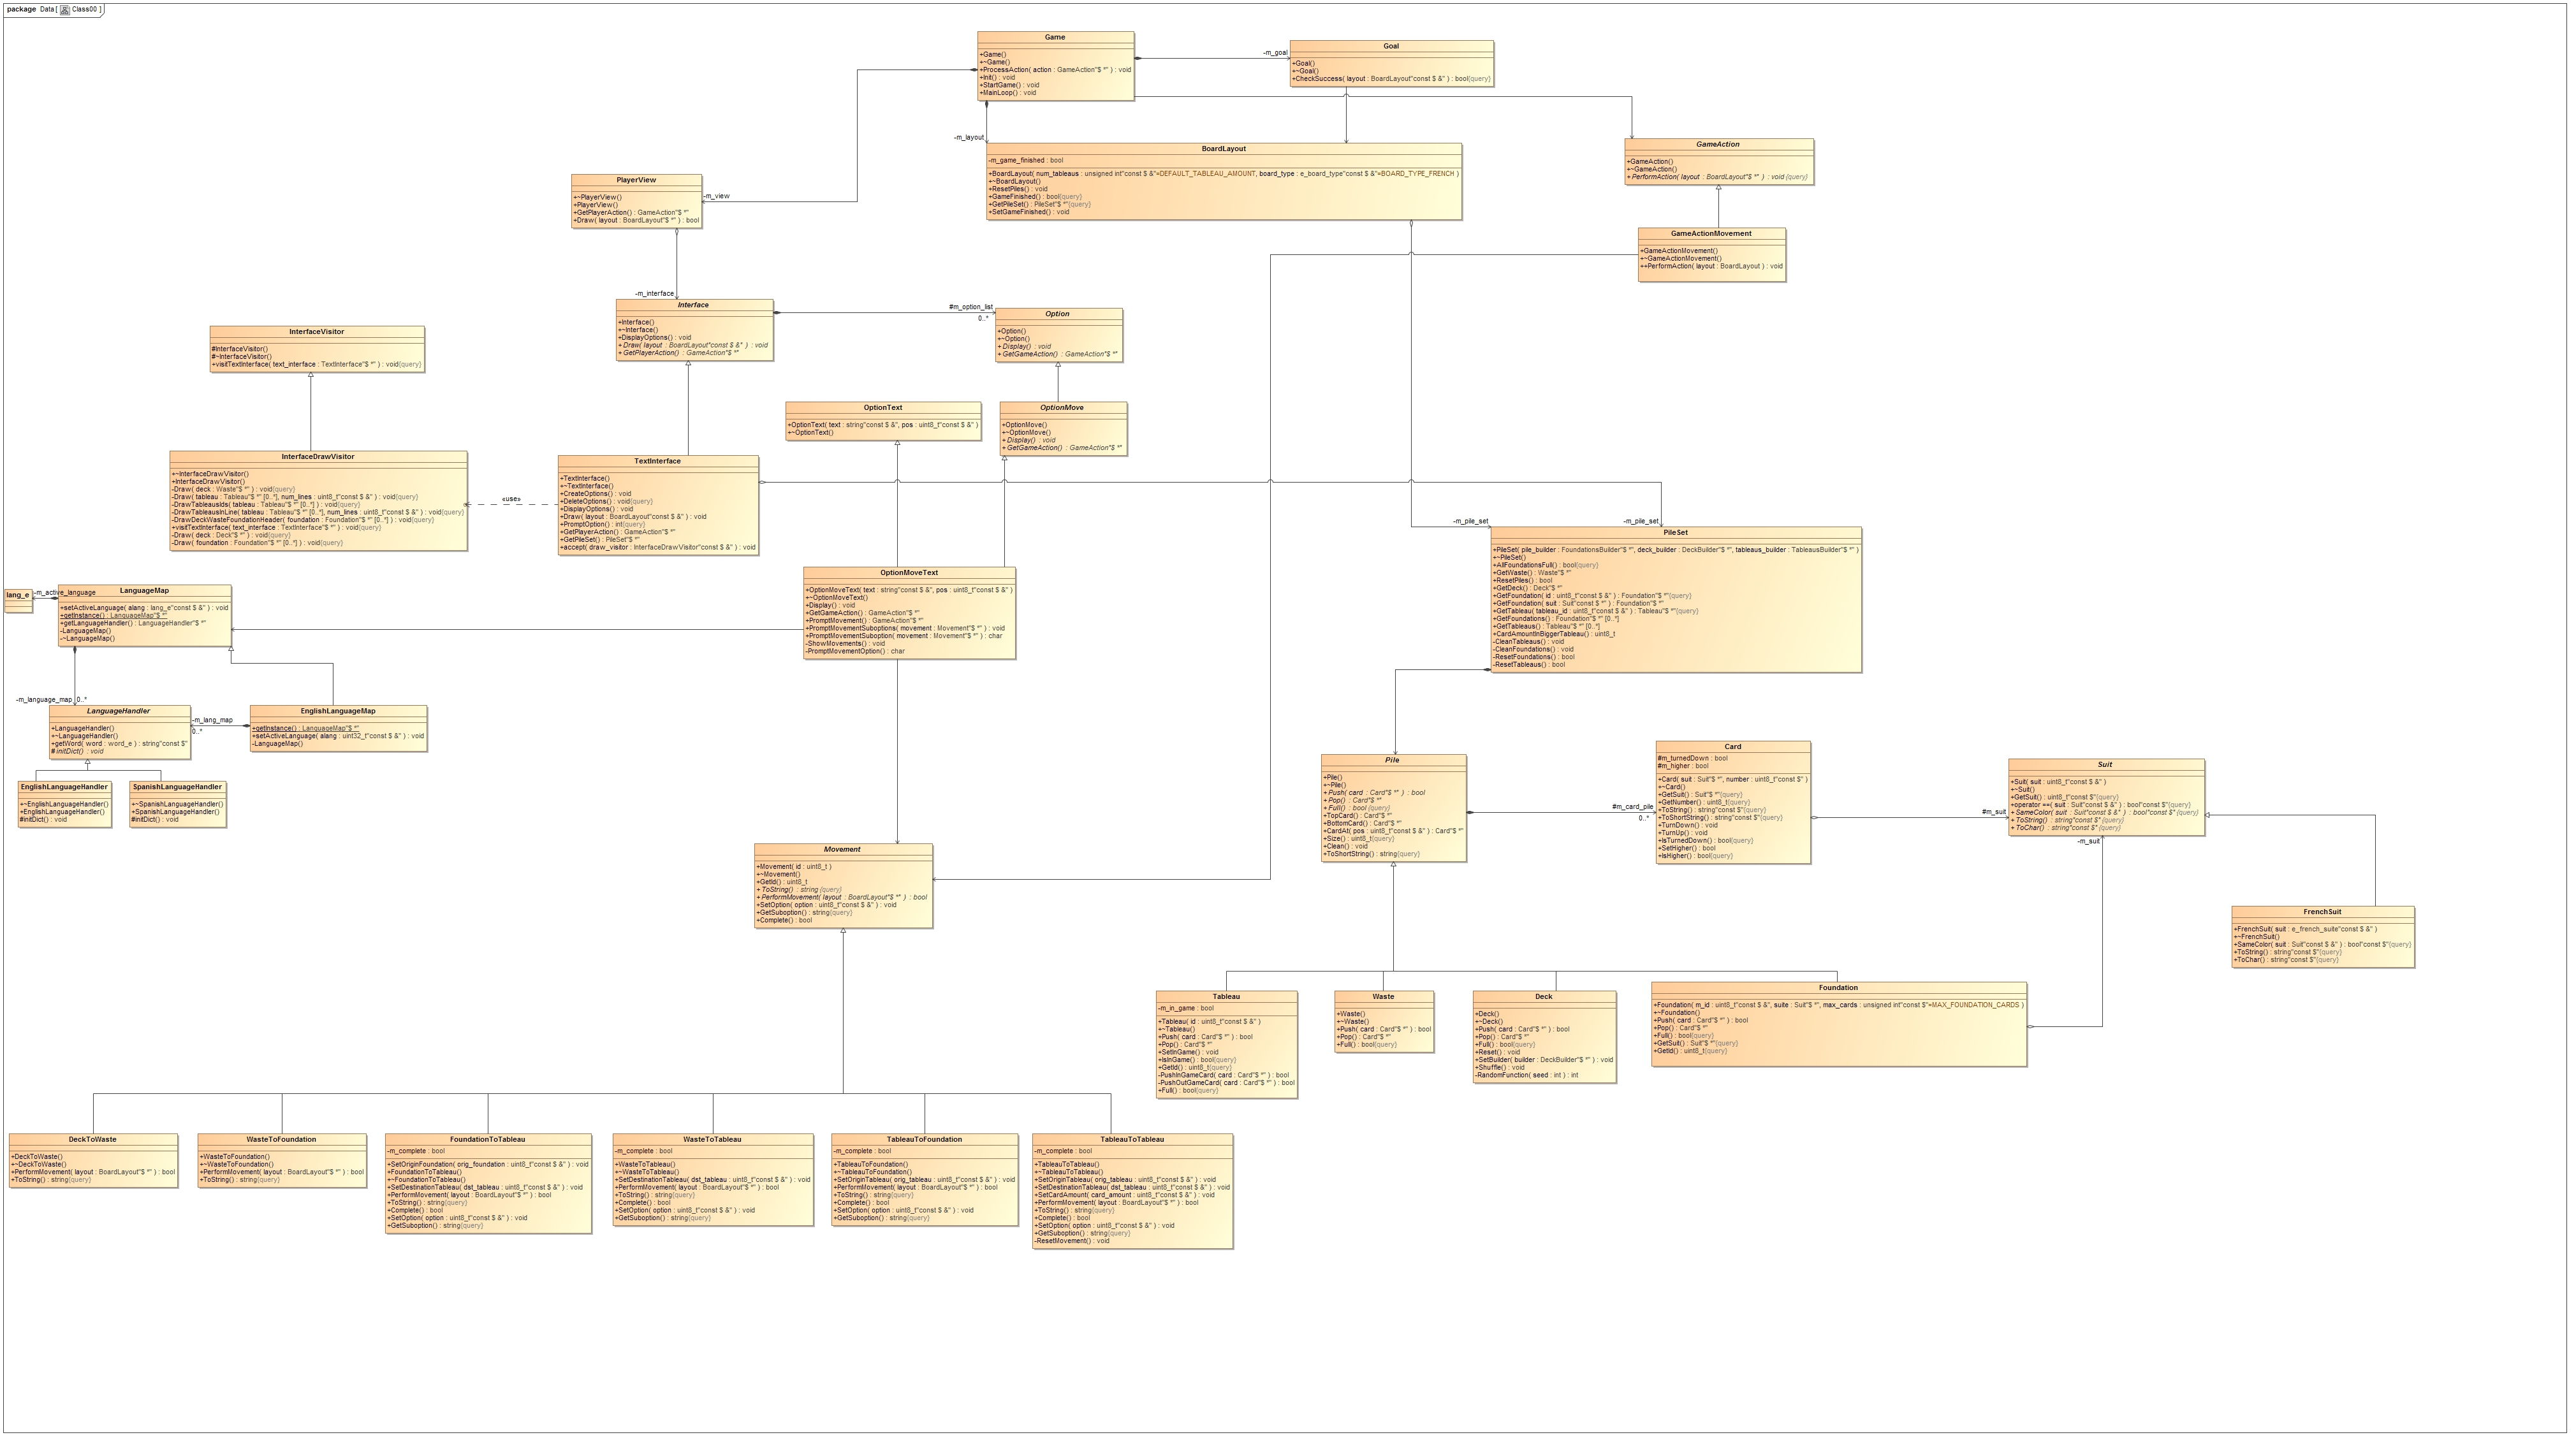
\includegraphics[scale=0.18]{Analysis/MoveCard00.jpg}
   \caption{Diagrama de Clases: ``Move Card''}
   \label{fig:movecard}
 \end{center}
 \end{figure}
\end{center}
\end{landscape}
\restoregeometry

\subsection{Diagramas de Interacción} 

Los diagramas de interacción permiten especificar, para cada caso de uso, las interacciones que se realizan a nivel de clase por cada caso de uso. Los siguientes diagramas muestran las principales interacciones para cada uno de los casos de uso:

\begin{center}
 \begin{figure}[H]
 \begin{center}
   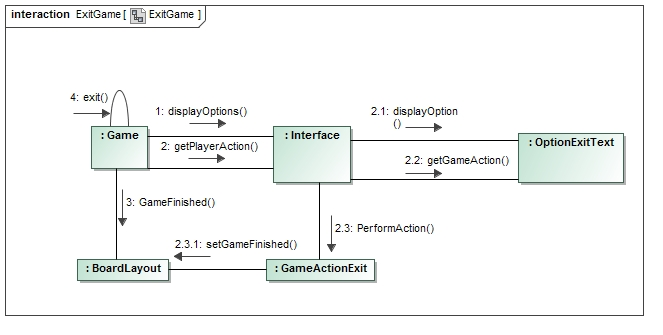
\includegraphics[width=16cm]{Analysis/ExitGameSequence00.jpg}
   \caption{Diagrama de Interacción: ``Exit Game''}
   \label{fig:exitgamesequence}
 \end{center}
 \end{figure}
\end{center}

\begin{center}
 \begin{figure}[H]
 \begin{center}
   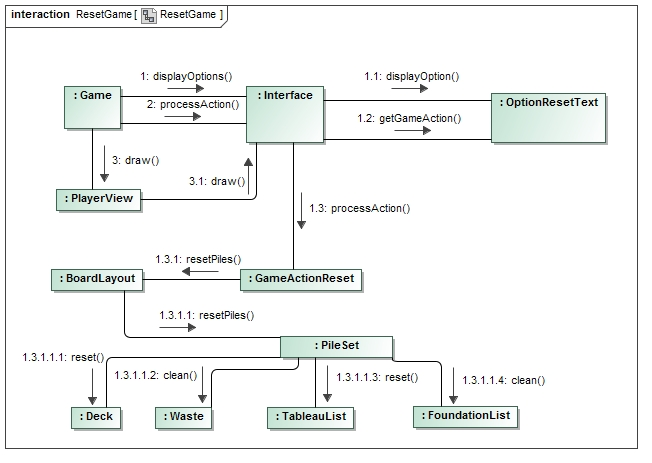
\includegraphics[width=16cm]{Analysis/ResetGameSequence00.jpg}
   \caption{Diagrama de Interacción: ``Start Game'' y ``Start New Game''}
   \label{fig:exitgamesequence}
 \end{center}
 \end{figure}
\end{center}

\begin{center}
 \begin{figure}[H]
 \begin{center}
   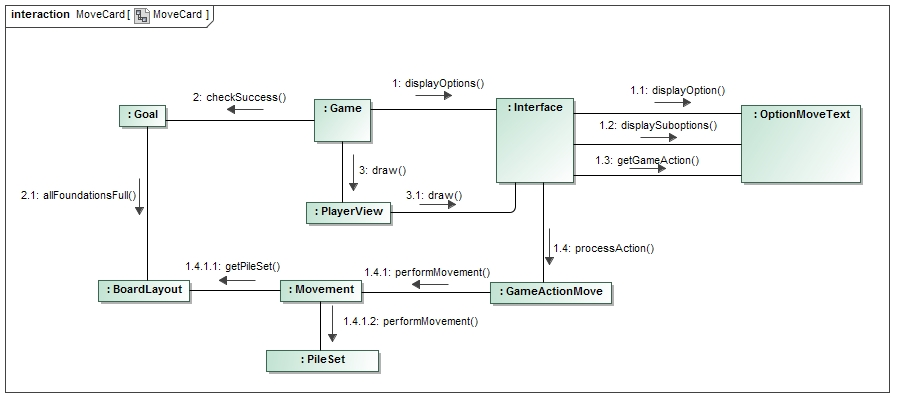
\includegraphics[width=17cm]{Analysis/MoveCardGenericSequence00.jpg}
   \caption{Diagrama de Interacción: ``Move Card''}
   \label{fig:movecardsequence}
 \end{center}
 \end{figure}
\end{center}

El último diagrama de secuencia, relativo a la interacción que se produce entre clases cuando se realiza el movimiento de una carta, está generalizado para todos los movimientos.

En realidad, en función del tipo de movimiento, se realizarán diversas acciones sobre la clase "PileSet". 
\end{document}
